%%%%%%%%%%%%%%%%%%%%%%%%%%%%%%%%%%%%%%%%%%%%%%%%%%%%%%%%%%%
\section{Anecdotal cases}
%%%%%%%%%%%%%%%%%%%%%%%%%%%%%%%%%%%%%%%%%%%%%%%%%%%%%%%%%%%
%
%
%%%%%%%%%%%%%%%%%%%%%%%%%%%%%%%%%%%%%%%%%%%%%%%%%%%%%%%%%%%
\subsection{Experimental design: the panacea}
%%%%%%%%%%%%%%%%%%%%%%%%%%%%%%%%%%%%%%%%%%%%%%%%%%%%%%%%%%%
%
%
\begin{frame}[t, negative]
	\subsectionpage
\end{frame}
%
%
\begin{frame}
	{Intervention}
	%
	\begin{columns}
		%
		\begin{column}{0.5\textwidth}
			%
			\begin{itemize}
				%
				\item Purpose: to keep a control on all the factors responsible for the outcome's variation \texcolort{blue}{(understand the system)}.
				%
				\item It is modeled by modifying the structural model (and causal diagram).
				%
				\item remember: $\pmb{V}=\{Z,X,Y\}$, $\pmb{U}=\{U_{z},U_{x},U_{y}\}$, and $\pmb{F}=\{f_{z},f_{x},f_{y}\}$.
				%
				\item Intervention on $X$ can be written in do-calculus\footnote{we are not delving into this (the usual suspects \cite{Pearl_1988, Pearl_2009, Pearl_et_al_2016, Pearl_et_al_2018})} as: $P(\pmb{V} \; | \; do(X=x))$.
				%
			\end{itemize}
			%
		\end{column}
		%
		\begin{column}{0.5\textwidth}  
			%
			\begin{equ}
				%
				M = \left\{ \begin{aligned} 
					Z \leftarrow & \; f_{z}(U_{z}) \\
					X \leftarrow & \; f_{x}(U_{x}) \\
					Y \leftarrow & \; f_{y}(X, Z, U_{y}) \\
					U \sim & \; P(\pmb{U})
				\end{aligned} \right
				%
				\caption*{(a) structural model}
			\end{equ}
			%
			\begin{figure}
				%
				\begin{tikzpicture}
					% nodes
					\node[formula] at (-2,0) {$x$};
					\node[formula] at (-1,-0.3) {$X$};
					\node[formula] at (1,1.5) {$U_{z}$};
					\node[formula] at (0,1) {$Z$};
					\node[formula] at (2,0) {$U_{y}$};
					\node[formula] at (1,-0.3) {$Y$};
					
					% paths
					\draw [{Circle [open]}-{latex}](-1.7,0)--(-1,0); % Ux->X
					\draw [{Circle}-{latex}](-1,0)--(0.9,0); % X->Y
					\draw [{Circle [open]}-{latex}{Circle}](1.7,0)--(0.9,0); % Uy->Y
					\draw [{Circle}-{latex}](0,0.8)--(0.9,0.1); % Z->Y
					\draw [{Circle [open]}-{latex}](0.9,1.3)--(0.1,0.8); % Uz->Z
				\end{tikzpicture}
				\caption*{(b) causal diagram}
			\end{figure}
			%
		\end{column}
		%
	\end{columns}
	%
\end{frame}
%
%
\begin{frame}
	{Effects of interest}
	%
	\begin{columns}
		%
		\begin{column}{0.5\textwidth}
			%
			\begin{enumerate}
				%
				\item Average causal effect: \\
				$\text{ACE}(x) = E[Y | do(x + 1)] - E[Y | do(x)]$
				%
				\item Controlled direct effect: \\
				$\text{CDE}(x, z) = E[Y | do(x + 1), do(z)] - E[Y | do(x), do(z)]$
				%
			\end{enumerate}
			%
			\heading{points to consider \alert{(more on part 3)}:}
			%
			\begin{itemize}
				%
				\item \textcolor{blue}{CDE} takes a particular relevance with \textcolor{blue}{observational data}.
				%
				\item There is also a distinction between \textcolor{blue}{total effect} and \textcolor{blue}{direct effect}.
				%
			\end{itemize}
			%
		\end{column}
		%
		\begin{column}{0.5\textwidth}  
			%
			\begin{equ}
				%
				M = \left\{ \begin{aligned} 
					Z \leftarrow & \; f_{z}(U_{z}) \\
					X \leftarrow & \; f_{x}(U_{x}) \\
					Y \leftarrow & \; f_{y}(X, Z, U_{y}) \\
					U \sim & \; P(\pmb{U})
				\end{aligned} \right
				%
				\caption*{(a) structural model}
			\end{equ}
			%
			\begin{figure}
				%
				\begin{tikzpicture}
					% nodes
					\node[formula] at (-2,0) {$x$};
					\node[formula] at (-1,-0.3) {$X$};
					\node[formula] at (1,1.5) {$U_{z}$};
					\node[formula] at (0,1) {$Z$};
					\node[formula] at (2,0) {$U_{y}$};
					\node[formula] at (1,-0.3) {$Y$};
					
					% paths
					\draw [{Circle [open]}-{latex}](-1.7,0)--(-1,0); % Ux->X
					\draw [{Circle}-{latex}](-1,0)--(0.9,0); % X->Y
					\draw [{Circle [open]}-{latex}{Circle}](1.7,0)--(0.9,0); % Uy->Y
					\draw [{Circle [color=red]}-{latex}](0,0.8)--(0.9,0.1); % Z->Y
					\draw [{Circle [open]}-{latex}](0.9,1.3)--(0.1,0.8); % Uz->Z
				\end{tikzpicture}
				\caption*{(b) causal diagram}
			\end{figure}
			%
		\end{column}
		%
	\end{columns}
	%
\end{frame}
%
%
%%%%%%%%%%%%%%%%%%%%%%%%%%%%%%%%%%%%%%%%%%%%%%%%%%%%%%%%%%%
\subsection{Fork bias: spurious relationships}
%%%%%%%%%%%%%%%%%%%%%%%%%%%%%%%%%%%%%%%%%%%%%%%%%%%%%%%%%%%
%
%
\begin{frame}[t, negative]
	\subsectionpage
\end{frame}
%
%
\begin{frame}
	{Fork bias: spurious relationships\footnote{extracted from \citet{McElreath_2020}, chapter 05 (p. 125)}}
	%
	\begin{columns}
		%
		\begin{column}{0.5\textwidth}
			%
			\heading{also known as}
			%
			\begin{itemize}
				%
				\item spurious association
				\item confounder
				%
			\end{itemize}
			%
			\heading{research question} 
			%
			\begin{itemize}
				%
				\item Does $M$ has a (direct) effect on $D$?
				%
			\end{itemize}
			%
			\heading{variables}
			%
			\begin{itemize}
				%
				\item A, median age at marriage
				\item M, marriage rate
				\item D, divorce rate
				%
			\end{itemize}
			%
		\end{column}
		%
		\begin{column}{0.5\textwidth}  
			%
			\begin{equ}
				%
				M = \left\{ \begin{aligned} 
					A \leftarrow & \; f_{a}(U_{a}) \\
					M \leftarrow & \; f_{m}(A,U_{m}) \\
					D \leftarrow & \; f_{d}(A, M, U_{d}) \\
					U \sim & \; P(\pmb{U})
				\end{aligned} \right
				%
				\caption*{(a) structural model}
			\end{equ}
			%
			\begin{figure}
				%
				\begin{tikzpicture}
					% nodes
					\node[formula] at (-2,0) {$U_{m}$};
					\node[formula] at (-1,-0.3) {$M$};
					\node[formula] at (1,1.5) {$U_{a}$};
					\node[formula] at (0,1) {$A$};
					\node[formula] at (2,0) {$U_{d}$};
					\node[formula] at (1,-0.3) {$D$};
					
					% paths
					\draw [{Circle [open]}-{latex}{Circle}](-1.7,0)--(-0.9,0); % Um->M
					\draw [red, -{latex}](-0.9,0)--(0.9,0); % M->D
					\draw [{Circle [open]}-{latex}{Circle}](1.7,0)--(0.9,0); % Ud->D
					\draw [{Circle [color=red]}-{latex}](0.1,0.8)--(-0.9,0.1); % A->M
					\draw [-{latex}](0.1,0.75)--(0.9,0.1); % A->D
					\draw [{Circle [open]}-{latex}](0.9,1.3)--(0.1,0.8); % Ua->A
				\end{tikzpicture}
				\caption*{(b) causal diagram}
			\end{figure}
			%
		\end{column}
		%
	\end{columns}
	%
\end{frame}
%
%
\begin{frame}
	{Simulation conventions}
	%
	\begin{columns}
		%
		\begin{column}{0.5\textwidth}
			%
			\heading{one way to defined it}
			%
			\begin{align*}
				%
				A = & \; U_{a} \; & U_{a} \sim & \; N(0, \sigma_{a})\\
				M = & \; \beta_{A} A + U_{m} \; & U_{m} \sim & \; N(0, \sigma_{a}) \\
				D = & \; \beta_{A} A + \beta_{M} M + U_{d} \; & U_{d} \sim & \; N(0, \sigma_{a})
			\end{align*}
			%
			%
			\heading{a more succinct way }
			%
			\begin{align*}
				%
				A \sim & \; N(0, \sigma_{a}) \\
				M \sim & \; N(\beta_{A} A, \sigma_{m}) \\
				D \sim & \; N(\beta_{A} A + \beta_{M} M, \sigma_{d}) 
			\end{align*}
			%
		\end{column}
		%
		\begin{column}{0.5\textwidth}  
			%
			\begin{equ}
				%
				M = \left\{ \begin{aligned} 
					A \leftarrow & \; f_{a}(U_{a}) \\
					M \leftarrow & \; f_{m}(A,U_{m}) \\
					D \leftarrow & \; f_{d}(A, M, U_{d}) \\
					U \sim & \; P(\pmb{U})
				\end{aligned} \right
				%
				\caption*{(a) structural model}
			\end{equ}
			%
			\begin{figure}
				%
				\begin{tikzpicture}
					% nodes
					\node[formula] at (-2,0) {$U_{m}$};
					\node[formula] at (-1,-0.3) {$M$};
					\node[formula] at (1,1.5) {$U_{a}$};
					\node[formula] at (0,1) {$A$};
					\node[formula] at (2,0) {$U_{d}$};
					\node[formula] at (1,-0.3) {$D$};
					
					% paths
					\draw [{Circle [open]}-{latex}{Circle}](-1.7,0)--(-0.9,0); % Um->M
					\draw [red, -{latex}](-0.9,0)--(0.9,0); % M->D
					\draw [{Circle [open]}-{latex}{Circle}](1.7,0)--(0.9,0); % Ud->D
					\draw [{Circle [color=red]}-{latex}](0.1,0.8)--(-0.9,0.1); % A->M
					\draw [-{latex}](0.1,0.75)--(0.9,0.1); % A->D
					\draw [{Circle [open]}-{latex}](0.9,1.3)--(0.1,0.8); % Ua->A
				\end{tikzpicture}
				\caption*{(b) causal diagram}
			\end{figure}
			%
		\end{column}
		%
	\end{columns}
	%
\end{frame}
%
%
\begin{frame}
	{Simulation setting}
	%
	\begin{columns}
		%
		\begin{column}{0.5\textwidth}
			%
			\heading{Implications}
			%
			\begin{itemize}
				%
				\item $\ndsep{M}{D} \;$
				\item $\ndsep{M}{D} \; | \; A$
				% 
			\end{itemize}
			%
			\heading{Specific definition}
			%
			\begin{align*}
				%
				A \sim & \; N(0, 1) \\
				M \sim & \; N(-A, 1) \\
				D \sim & \; N(-A + 0 \times M, 1)
				% 
			\end{align*}
			%
			\heading{R code}
			
			\begin{codesnippet}[\textwidth]
				n = 100 \\
				A = rnorm( n ) \\
				M = rnorm( n , mean=-A ) \\
				D = rnorm( n , mean=-A + 0*M ) 
			\end{codesnippet}
			%
		\end{column}
		%
		\begin{column}{0.5\textwidth}  
			%
			\begin{equ}
				%
				M = \left\{ \begin{aligned} 
					A \leftarrow & \; f_{a}(U_{a}) \\
					M \leftarrow & \; f_{m}(A,U_{m}) \\
					D \leftarrow & \; f_{d}(A, U_{d}) \\
					U \sim & \; P(\pmb{U})
				\end{aligned} \right
				%
				\caption*{(a) structural model}
			\end{equ}
			%
			\begin{figure}
				%
				\begin{tikzpicture}
					% nodes
					\node[formula] at (-2,0) {$U_{m}$};
					\node[formula] at (-1,-0.3) {$M$};
					\node[formula] at (1,1.5) {$U_{a}$};
					\node[formula] at (0,1) {$A$};
					\node[formula] at (2,0) {$U_{d}$};
					\node[formula] at (1,-0.3) {$D$};
					
					% paths
					\draw [{Circle [open]}-{latex}{Circle}](-1.7,0)--(-0.9,0); % Um->M
					%\draw [red, -{latex}](-0.9,0)--(0.9,0); % M->D
					\draw [{Circle [open]}-{latex}{Circle}](1.7,0)--(0.9,0); % Ud->D
					\draw [{Circle [color=red]}-{latex}](0.1,0.8)--(-0.9,0.1); % A->M
					\draw [-{latex}](0.1,0.75)--(0.9,0.1); % A->D
					\draw [{Circle [open]}-{latex}](0.9,1.3)--(0.1,0.8); % Ua->A
				\end{tikzpicture}
				\caption*{(b) causal diagram}
			\end{figure}
			%
		\end{column}
		%
	\end{columns}
	%
\end{frame}
%
%
\begin{lhframe}[rhgraphic={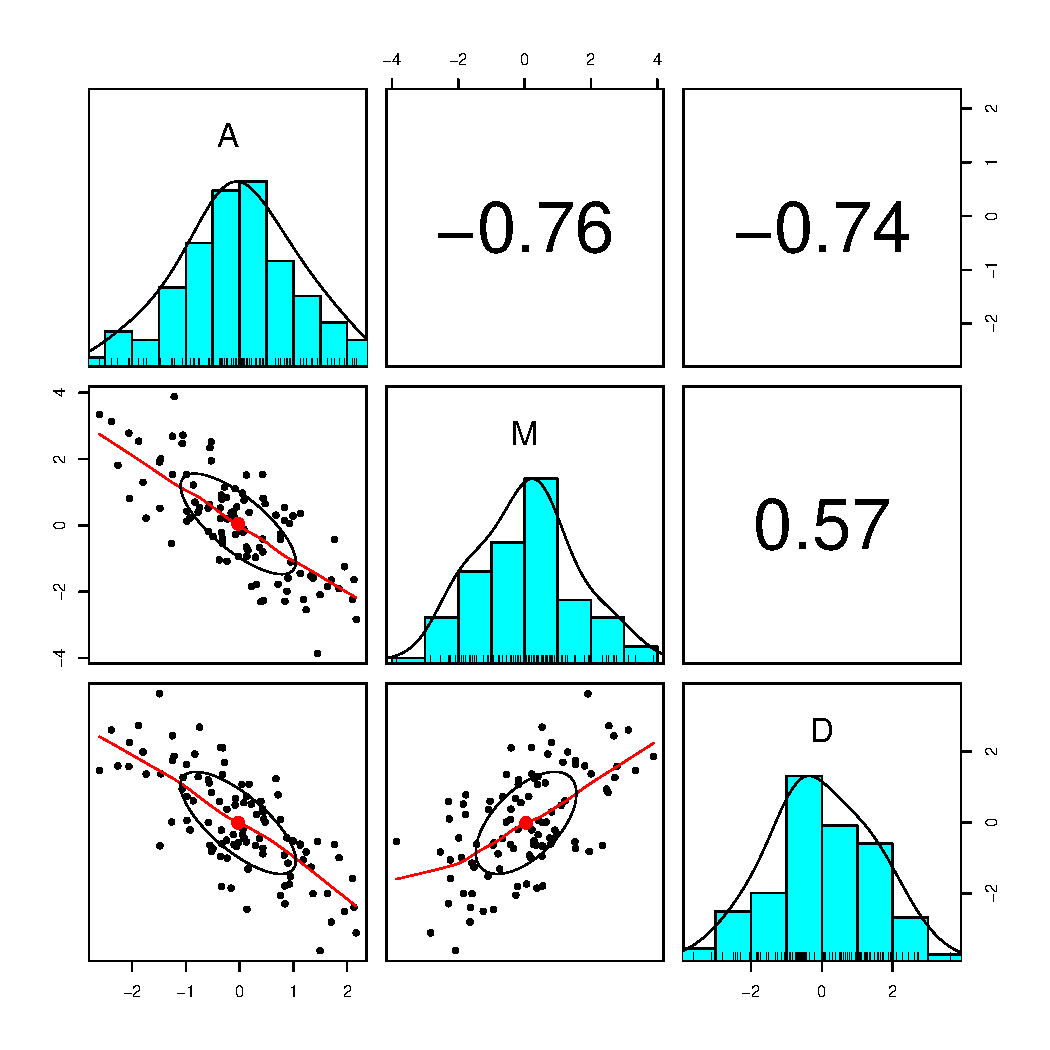
\includegraphics[scale=0.4]{spurious.pdf}}]
	{What we see?}
	{and what we might decide}
	
	\heading{Two regressions, one result}
	
	\begin{codesnippet}[\textwidth]
		summary(lm(D \command{~} M, data=d)) \\ \\
		> Coefficients: \\
		> Estimate Std. Error t value Pr(>|t|) \\
		> (Intercept) -0.03364    0.11863  -0.284    0.777 \\
		> M            0.54561    0.07848   6.952 4.03e-10 *** \\ 
	\end{codesnippet}
	%
\end{lhframe}
%
%
\begin{frame}[t]
	{Result}
	
	Frishc-Waugh-Lovell
	Backdoor criterion on bad controls paper (p. 18)
\end{frame}
%
%
\begin{frame}[t]
	{What is going on?}
\end{frame}
%
%
